%%Chci udelat obrazky pro situace k dukazy nezavislosti sousedstvi N(u) pro vrchol z min vertex coveru

\documentclass[tikz,border=3mm]{standalone}
\usetikzlibrary{shapes,snakes}
\usetikzlibrary{backgrounds}
\usetikzlibrary{calc}
\def\width{1.65}
\def\height{-2.5}
\begin{document}
        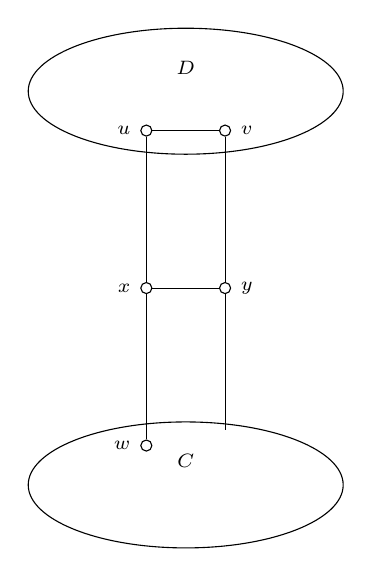
\begin{tikzpicture}

		\tikzstyle{vertex}  = [circle, minimum width=4pt, draw, inner sep=0pt, fill=white]
		\node [vertex, label=left:{\scriptsize$x$}](x) at (1, 3) {};
		\node [vertex, label=right:{\scriptsize$y$}](y) at (2, 3) {};
		\node [vertex, label=left:{\scriptsize$u$}](u) at (1, 5) {};
                \node [vertex, label=right:{\scriptsize$v$}](v) at (2, 5) {};
		\node [vertex, label=left:{\scriptsize$w$}](w) at (1, 1) {};

		%%Components C and D
		\draw ({1.5}, 5.5) ellipse (2cm and 0.8cm);
		\draw ({1.5}, 0.5) ellipse (2cm and 0.8cm);
		%%Labels for components C and D
		\node (d) at ({1.5}, 5.8) {\scriptsize$D$};
		\node (c) at ({1.5}, 0.8) {\scriptsize$C$};

		
		\draw (x)--(y)--(v)--(u)--(x);
		\draw (x)--(w);
		\draw (y)--(2,1.2);
	\end{tikzpicture}

	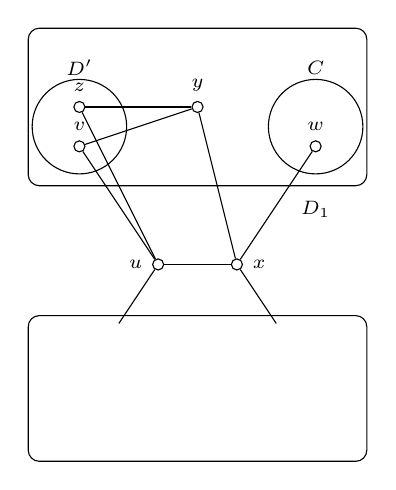
\begin{tikzpicture}
	\tikzstyle{vertex}  = [circle, minimum width=4pt, draw, inner sep=0pt, fill=white]
	\node [vertex, label=left:{\scriptsize$u$}](u) at (1, 3) {};
        \node [vertex, label=right:{\scriptsize$x$}](x) at (2, 3) {};
	\node [vertex, label=above:{\scriptsize$y$}](y) at ($(x)!0.5!(u) + (0, 2)$) {};
	\node [vertex, label=above:{\scriptsize$z$}](z) at ($(y) + (-1.5, 0)$) {};
	\node [vertex, label=above:{\scriptsize$v$}](v) at ($(z) + (0, -0.5)$) {};
	\node [vertex, label=above:{\scriptsize$w$}](w) at ($(y) + (1.5, -0.5)$) {};
	\node (z2) at ($(y) + (1.5, 0)$) {};
	
	\draw[rounded corners] ($(u) + (-\width, {\height})$) rectangle ($(x) + (\width, -0.65)$) {};
	\draw[rounded corners] ($(u) + (-\width, 1)$) rectangle ($(x) + (\width, -\height + 0.5)$) {};
	\draw ($(z)!0.5!(v)$) ellipse (0.6cm and 0.6cm);
	\draw ($(z2)!0.5!(w)$) ellipse (0.6cm and 0.6cm);
	%%Components labels
	\node (ld) at ($(z) + (0, 0.5)$) {\scriptsize$D'$};
	\node (lc) at ($(z2) + (0, 0.5)$) {\scriptsize$C$};
	\node (lD1) at ($(w) + (0, -0.8)$) {\scriptsize$D_1$};

	\draw (x)--(w);
	\draw (u)--(x);
	\draw (x)--(y);
	\draw (y)--(z);
	\draw (z)--(u);
	\draw (u)--(v);
	\draw (v)--(y);

	\draw (x)--($(x) + (0.5, -0.75)$);
	\draw (u)--($(u) + (-0.5, -0.75)$);
	\end{tikzpicture}

\end{document}
